\documentclass[11pt,fleqn]{book} % Default font size and left-justified equations

%%----------------------------------------------------------------------------------------
%	PREAMBLE
%%%%%%%%%%%%%%%%%%%%%%%%%%%%%%%%%%%%%%%%%
% The Legrand Orange Book
% Structural Definitions File
% Version 2.0 (9/2/15)
%
% Original author:
% Mathias Legrand (legrand.mathias@gmail.com) with modifications by:
% Vel (vel@latextemplates.com)
% 
% This file has been downloaded from:
% http://www.LaTeXTemplates.com
%
% License:
% CC BY-NC-SA 3.0 (http://creativecommons.org/licenses/by-nc-sa/3.0/)
%
%%%%%%%%%%%%%%%%%%%%%%%%%%%%%%%%%%%%%%%%%

\usepackage{todonotes}

%%----------------------------------------------------------------------------------------
%	VARIOUS REQUIRED PACKAGES AND CONFIGURATIONS
\usepackage[top=3cm,bottom=3cm,left=3cm,right=3cm,headsep=10pt,a4paper]{geometry} % Page margins
\usepackage{graphicx} % Required for including pictures
\graphicspath{{Resources/media/pictures/}{Resources/media/figures/}{Resources/media/pictures/chapterHeadings/}} % Specifies the directory where pictures are stored
\usepackage{lipsum} % Inserts dummy text
\usepackage{tikz} % Required for drawing custom shapes
\usepackage[english]{babel} % English language/hyphenation
\usepackage{enumitem} % Customize lists
\usepackage{dcolumn} % I ADDED
\setlist{nolistsep} % Reduce spacing between bullet points and numbered lists
\usepackage{booktabs} % Required for nicer horizontal rules in tables
\usepackage{xcolor} % Required for specifying colors by name
%% Colors from original templates
\definecolor{ocre}{RGB}{243,102,25} % Define the orange color used for highlighting throughout the book
\definecolor{carolinablue}{RGB}{168,192,252}
%% Virginia Tech Color Palette
%  https://vt.edu/brand.html
\definecolor{VTchicagoMaroon}{RGB}{134,31,65}
\definecolor{VTburntOrange}{RGB}{232,119,34}
\definecolor{VTyardlineWhite}{RGB}{255,255,255}
\definecolor{VThokieStone}{RGB}{117,120,123}
\definecolor{VTpylonPurple}{RGB}{100,38,103}
\definecolor{VTboundlessPink}{RGB}{206,0,88}
\definecolor{VTvirginiaSunset}{RGB}{237,139,0}
\definecolor{VTtriumphantYellow}{RGB}{247,234,72}
\definecolor{VTsustainableTeal}{RGB}{80,133,144}
\definecolor{VTvibrantTurquoise}{RGB}{44,213,196}
\definecolor{VTlandgrantGrey}{RGB}{215,210,203}
\definecolor{VTskipperSmoke}{RGB}{229,225,230}
\definecolor{VTburntOrangeWEB}{RGB}{197,69,20}
\definecolor{VTcadetBlue}{RGB}{11,61,110}
% team color codes
% https://teamcolorcodes.com/virginia-tech-hokies-color-codes/
\definecolor{VTchicagoMaroonTEAM}{RGB}{106,44,62}
\definecolor{VTburntOrangeTEAM}{RGB}{207,69,32}

%%----------------------------------------------------------------------------------------
%	LOADING DATA FOR PROBLEMS & SOLUTIONS
\usepackage{datatool} % I ADDED (for reading csv's)
\newcommand{\V}[1]{\DTLfetch{Solutions01}{ch_pr_var}{#1}{\whichBook}} % needs to be renewed every Problems##.tex file for new chapter
\newcommand{\File}[1]{Problems/Solutions/csvFiles/Solutions#1.csv}
\IfFileExists{\File{01}}{\DTLloaddb{Solutions01}{\File{01}}}{\relax}
\IfFileExists{\File{02}}{\DTLloaddb{Solutions02}{\File{02}}}{\relax}
\IfFileExists{\File{03}}{\DTLloaddb{Solutions03}{\File{03}}}{\relax}
\IfFileExists{\File{04}}{\DTLloaddb{Solutions04}{\File{04}}}{\relax}
\IfFileExists{\File{05}}{\DTLloaddb{Solutions05}{\File{05}}}{\relax}
\IfFileExists{\File{06}}{\DTLloaddb{Solutions06}{\File{06}}}{\relax}
\IfFileExists{\File{07}}{\DTLloaddb{Solutions07}{\File{07}}}{\relax}
\IfFileExists{\File{08}}{\DTLloaddb{Solutions08}{\File{08}}}{\relax}
\IfFileExists{\File{09}}{\DTLloaddb{Solutions09}{\File{09}}}{\relax}
\IfFileExists{\File{10}}{\DTLloaddb{Solutions10}{\File{10}}}{\relax}
\IfFileExists{\File{11}}{\DTLloaddb{Solutions11}{\File{11}}}{\relax}
\IfFileExists{\File{12}}{\DTLloaddb{Solutions12}{\File{12}}}{\relax}
\IfFileExists{\File{13}}{\DTLloaddb{Solutions13}{\File{13}}}{\relax}
\IfFileExists{\File{14}}{\DTLloaddb{Solutions14}{\File{14}}}{\relax}
\IfFileExists{\File{15}}{\DTLloaddb{Solutions15}{\File{15}}}{\relax}
\IfFileExists{\File{16}}{\DTLloaddb{Solutions16}{\File{16}}}{\relax}
\IfFileExists{\File{17}}{\DTLloaddb{Solutions17}{\File{17}}}{\relax}
\IfFileExists{\File{18}}{\DTLloaddb{Solutions18}{\File{18}}}{\relax}
\IfFileExists{\File{19}}{\DTLloaddb{Solutions19}{\File{19}}}{\relax}
\IfFileExists{\File{20}}{\DTLloaddb{Solutions20}{\File{20}}}{\relax}
\IfFileExists{\File{21}}{\DTLloaddb{Solutions21}{\File{21}}}{\relax}

%%--------------------------------------------------------------------------------------
%	FONTS
\usepackage{draftwatermark}
\SetWatermarkText{DRAFT}
\SetWatermarkScale{1}
\usepackage{avant} % Use the Avantgarde font for headings
%\usepackage{times} % Use the Times font for headings
\usepackage{mathptmx} % Use the Adobe Times Roman as the default text font together with math symbols from the Symbol, Chancery and Computer Modern fonts
\usepackage{microtype} % Slightly tweak font spacing for aesthetics
\usepackage[utf8]{inputenc} % Required for including letters with accents
\usepackage[T1]{fontenc} % Use 8-bit encoding that has 256 glyphs
\usepackage{dirtytalk} % I ADDED
\newcommand{\RomanNumeralCaps}[1]
    {\MakeUppercase{\romannumeral #1}} % I ADDED 
    
%%----------------------------------------------------------------------------------------
%	BIBLIOGRAPHY AND INDEX
\usepackage{csquotes} % I ADDED, recommended 
\usepackage[title]{appendix} % I ADDED, for appendix labelling
\usepackage[style=numeric,citestyle=numeric,sorting=nyt,sortcites=true,autopunct=true,autolang=hyphen,hyperref=true,abbreviate=false,backend=biber]{biblatex} % I removed backref=true
\addbibresource{bibliography.bib} % BibTeX bibliography file
\defbibheading{bibempty}{}
\usepackage{calc} % For simpler calculation - used for spacing the index letter headings correctly
\usepackage{makeidx} % Required to make an index
\makeindex % Tells LaTeX to create the files required for indexing

%%----------------------------------------------------------------------------------------
%	MAIN TABLE OF CONTENTS
\usepackage{titletoc} % Required for manipulating the table of contents
\contentsmargin{0cm} % Removes the default margin
% Part text styling
\titlecontents{part}[0cm]
{\addvspace{20pt}\centering\large\bfseries}
{}
{}
{}
% Chapter text styling
\titlecontents{chapter}[1.25cm] % Indentation
{\addvspace{12pt}\large\sffamily\bfseries} % Spacing and font options for chapters
{\color{carolinablue!60}\contentslabel[\Large\thecontentslabel]{1.25cm}\color{carolinablue}} % Chapter number
{\color{carolinablue}}  
{\color{carolinablue!60}\normalsize\;\titlerule*[.5pc]{.}\;\thecontentspage} % Page number
% Section text styling
\titlecontents{section}[1.25cm] % Indentation
{\addvspace{3pt}\sffamily\bfseries} % Spacing and font options for sections
{\contentslabel[\thecontentslabel]{1.25cm}} % Section number
{}
{\hfill\color{black}\thecontentspage} % Page number
[]
% Subsection text styling
\titlecontents{subsection}[1.25cm] % Indentation
{\addvspace{1pt}\sffamily\small} % Spacing and font options for subsections
{\contentslabel[\thecontentslabel]{1.25cm}} % Subsection number
{}
{\ \titlerule*[.5pc]{.}\;\thecontentspage} % Page number
[]
% List of figures
\titlecontents{figure}[0em]
{\addvspace{-5pt}\sffamily}
{\thecontentslabel\hspace*{1em}}
{}
{\ \titlerule*[.5pc]{.}\;\thecontentspage}
[]
% List of tables
\titlecontents{table}[0em]
{\addvspace{-5pt}\sffamily}
{\thecontentslabel\hspace*{1em}}
{}
{\ \titlerule*[.5pc]{.}\;\thecontentspage}
[]

%%----------------------------------------------------------------------------------------
%	MINI TABLE OF CONTENTS IN PART HEADS
% Chapter text styling
\titlecontents{lchapter}[-7em] % Indenting
{\addvspace{15pt}\large\sffamily\bfseries} % Spacing and font options for chapters
{\color{carolinablue}\contentslabel[\Large\thecontentslabel]{1.25cm}\color{carolinablue}} % Chapter number
{}  
{\color{carolinablue}\normalsize\sffamily\bfseries\titlerule*[1pc]{.}\thecontentspage} % Page number
% Section text styling
\titlecontents{lsection}[-7em] % Indenting
{\sffamily\small} % Spacing and font options for sections
{\contentslabel[\thecontentslabel]{1.25cm}} % Section number
{}
{}
% Subsection text styling
\titlecontents{lsubsection}[.5em] % Indentation
{\normalfont\footnotesize\sffamily} % Font settings
{}
{}
{}

%%----------------------------------------------------------------------------------------
%	PAGE HEADERS
\usepackage{fancyhdr} % Required for header and footer configuration
\pagestyle{fancy}
\renewcommand{\chaptermark}[1]{\markboth{\sffamily\normalsize\bfseries\chaptername\ \thechapter.\ #1}{}} % Chapter text font settings
\renewcommand{\sectionmark}[1]{\markright{\sffamily\normalsize\thesection\hspace{5pt}#1}{}} % Section text font settings
\fancyhf{} \fancyhead[LE,RO]{\sffamily\normalsize\thepage} % Font setting for the page number in the header
\fancyhead[LO]{\rightmark} % Print the nearest section name on the left side of odd pages
\fancyhead[RE]{\leftmark} % Print the current chapter name on the right side of even pages
\renewcommand{\headrulewidth}{0.5pt} % Width of the rule under the header
\addtolength{\headheight}{2.5pt} % Increase the spacing around the header slightly
\renewcommand{\footrulewidth}{0pt} % Removes the rule in the footer
\fancypagestyle{plain}{\fancyhead{}\renewcommand{\headrulewidth}{0pt}} % Style for when a plain pagestyle is specified
% Removes the header from odd empty pages at the end of chapters
\makeatletter
\renewcommand{\cleardoublepage}{
%\clearpage\ifodd\c@page\else % I COMMENTED OUT
\hbox{}
\vspace*{\fill}
\thispagestyle{empty}
\newpage
%\fi % I COMMENTED OUT
}

%%----------------------------------------------------------------------------------------
%	THEOREM STYLES
\usepackage{amsmath,amsfonts,amssymb,amsthm} % For math equations, theorems, symbols, etc
\newcommand{\intoo}[2]{\mathopen{]}#1\,;#2\mathclose{[}}
\newcommand{\ud}{\mathop{\mathrm{{}d}}\mathopen{}}
\newcommand{\intff}[2]{\mathopen{[}#1\,;#2\mathclose{]}}
\newtheorem{notation}{Notation}[chapter]
% Boxed/framed environments
\newtheoremstyle{carolinabluenumbox}% % Theorem style name
{0pt}% Space above
{0pt}% Space below
{\normalfont}% % Body font
{}% Indent amount
{\small\bf\sffamily\color{carolinablue}}% % Theorem head font
{\;}% Punctuation after theorem head
{0.25em}% Space after theorem head
{\small\sffamily\color{carolinablue}\thmname{#1}\nobreakspace\thmnumber{\@ifnotempty{#1}{}\@upn{#2}}% Theorem text (e.g. Theorem 2.1)
\thmnote{\nobreakspace\the\thm@notefont\sffamily\bfseries\color{black}---\nobreakspace#3.}} % Optional theorem note
\renewcommand{\qedsymbol}{$\blacksquare$}% Optional qed square
\newtheoremstyle{blacknumex}% Theorem style name
{5pt}% Space above
{5pt}% Space below
{\normalfont}% Body font
{} % Indent amount
{\small\bf\sffamily}% Theorem head font
{\;}% Punctuation after theorem head
{0.25em}% Space after theorem head
{\small\sffamily{\tiny\ensuremath{\blacksquare}}\nobreakspace\thmname{#1}\nobreakspace\thmnumber{\@ifnotempty{#1}{}\@upn{#2}}% Theorem text (e.g. Theorem 2.1)
\thmnote{\nobreakspace\the\thm@notefont\sffamily\bfseries---\nobreakspace#3.}}% Optional theorem note
\newtheoremstyle{blacknumbox} % Theorem style name
{0pt}% Space above
{0pt}% Space below
{\normalfont}% Body font
{}% Indent amount
{\small\bf\sffamily}% Theorem head font
{\;}% Punctuation after theorem head
{0.25em}% Space after theorem head
{\small\sffamily\thmname{#1}\nobreakspace\thmnumber{\@ifnotempty{#1}{}\@upn{#2}}% Theorem text (e.g. Theorem 2.1)
\thmnote{\nobreakspace\the\thm@notefont\sffamily\bfseries---\nobreakspace#3.}}% Optional theorem note
% Non-boxed/non-framed environments
\newtheoremstyle{carolinabluenum}% % Theorem style name
{5pt}% Space above
{5pt}% Space below
{\normalfont}% % Body font
{}% Indent amount
{\small\bf\sffamily\color{carolinablue}}% % Theorem head font
{\;}% Punctuation after theorem head
{0.25em}% Space after theorem head
{\small\sffamily\color{carolinablue}\thmname{#1}\nobreakspace\thmnumber{\@ifnotempty{#1}{}\@upn{#2}}% Theorem text (e.g. Theorem 2.1)
\thmnote{\nobreakspace\the\thm@notefont\sffamily\bfseries\color{black}---\nobreakspace#3.}} % Optional theorem note
\renewcommand{\qedsymbol}{$\blacksquare$}% Optional qed square
\makeatother
% Defines the theorem text style for each type of theorem to one of the three styles above
\newcounter{dummy} 
\numberwithin{dummy}{section}
\theoremstyle{carolinabluenumbox}
\newtheorem{theoremeT}[dummy]{Theorem}
\newtheorem{problem}{Problem}[chapter]
%%%
%% For organizing PQE's and their solutions (I added) 
% allows separate publication, even with problem and solution together in text
% http://ctan.math.washington.edu/tex-archive/macros/latex/contrib/exsol/exsol.pdf
% \def\solutionname{Solution \thechapter.\arabic{exercise}} % failed
\usepackage[copyexercisesinsolutions]{exsol}
\renewcommand{\exercisesname}{} % just use standard header
\renewcommand{\exercisename}{Problem}
\renewcommand{\theexercise}{\thechapter.\arabic{exercise}}
%
%%
%%%
\newtheorem{exerciseT}{Exercise}[chapter]
\theoremstyle{blacknumex}
\newtheorem{exampleT}{Example}[chapter]
\theoremstyle{blacknumbox}
\newtheorem{vocabulary}{Vocabulary}[chapter]
\newtheorem{definitionT}{Definition}[section]
\newtheorem{corollaryT}[dummy]{Corollary}
\theoremstyle{carolinabluenum}
\newtheorem{proposition}[dummy]{Proposition}

%%----------------------------------------------------------------------------------------
%	DEFINITION OF COLORED BOXES
\RequirePackage[framemethod=default]{mdframed} % Required for creating the theorem, definition, exercise and corollary boxes
% Theorem box
\newmdenv[skipabove=7pt,
skipbelow=7pt,
backgroundcolor=black!5,
linecolor=carolinablue,
innerleftmargin=5pt,
innerrightmargin=5pt,
innertopmargin=5pt,
leftmargin=0cm,
rightmargin=0cm,
innerbottommargin=5pt]{tBox}
% Exercise box	  
\newmdenv[skipabove=7pt,
skipbelow=7pt,
rightline=false,
leftline=true,
topline=false,
bottomline=false,
backgroundcolor=carolinablue!10,
linecolor=carolinablue,
innerleftmargin=5pt,
innerrightmargin=5pt,
innertopmargin=5pt,
innerbottommargin=5pt,
leftmargin=0cm,
rightmargin=0cm,
linewidth=4pt]{eBox}	
% Definition box
\newmdenv[skipabove=7pt,
skipbelow=7pt,
rightline=false,
leftline=true,
topline=false,
bottomline=false,
linecolor=carolinablue,
innerleftmargin=5pt,
innerrightmargin=5pt,
innertopmargin=0pt,
leftmargin=0cm,
rightmargin=0cm,
linewidth=4pt,
innerbottommargin=0pt]{dBox}	
% Corollary box
\newmdenv[skipabove=7pt,
skipbelow=7pt,
rightline=false,
leftline=true,
topline=false,
bottomline=false,
linecolor=gray,
backgroundcolor=black!5,
innerleftmargin=5pt,
innerrightmargin=5pt,
innertopmargin=5pt,
leftmargin=0cm,
rightmargin=0cm,
linewidth=4pt,
innerbottommargin=5pt]{cBox}
% Creates an environment for each type of theorem and assigns it a theorem text style from the "Theorem Styles" section above and a colored box from above
\newenvironment{theorem}{\begin{tBox}\begin{theoremeT}}{\end{theoremeT}\end{tBox}}
% (I added) exercise -> exercise_original
\newenvironment{exercise_original}{\begin{eBox}\begin{exerciseT}}{\hfill{\color{carolinablue}\tiny\ensuremath{\blacksquare}}\end{exerciseT}\end{eBox}}				  
\newenvironment{definition}{\begin{dBox}\begin{definitionT}}{\end{definitionT}\end{dBox}}	
\newenvironment{example}{\begin{exampleT}}{\hfill{\tiny\ensuremath{\blacksquare}}\end{exampleT}}		
\newenvironment{corollary}{\begin{cBox}\begin{corollaryT}}{\end{corollaryT}\end{cBox}}	

%%----------------------------------------------------------------------------------------
%	REMARK ENVIRONMENT
\newenvironment{remark}{\par\vspace{10pt}\small % Vertical white space above the remark and smaller font size
\begin{list}{}{
\leftmargin=35pt % Indentation on the left
\rightmargin=25pt}\item\ignorespaces % Indentation on the right
\makebox[-2.5pt]{\begin{tikzpicture}[overlay]
\node[draw=carolinablue!60,line width=1pt,circle,fill=carolinablue!25,font=\sffamily\bfseries,inner sep=2pt,outer sep=0pt] at (-15pt,0pt){\textcolor{carolinablue}{R}};\end{tikzpicture}} % Orange R in a circle
\advance\baselineskip -1pt}{\end{list}\vskip5pt} % Tighter line spacing and white space after remark
%%----------------------------------------------------------------------------------------
%	SECTION NUMBERING IN THE MARGIN
%%----------------------------------------------------------------------------------------
\makeatletter
\renewcommand{\@seccntformat}[1]{\llap{\textcolor{carolinablue}{\csname the#1\endcsname}\hspace{1em}}}                    
\renewcommand{\section}{\@startsection{section}{1}{\z@}
{-4ex \@plus -1ex \@minus -.4ex}
{1ex \@plus.2ex }
{\normalfont\large\sffamily\bfseries}}
\renewcommand{\subsection}{\@startsection {subsection}{2}{\z@}
{-3ex \@plus -0.1ex \@minus -.4ex}
{0.5ex \@plus.2ex }
{\normalfont\sffamily\bfseries}}
\renewcommand{\subsubsection}{\@startsection {subsubsection}{3}{\z@}
{-2ex \@plus -0.1ex \@minus -.2ex}
{.2ex \@plus.2ex }
{\normalfont\small\sffamily\bfseries}}                        
\renewcommand\paragraph{\@startsection{paragraph}{4}{\z@}
{-2ex \@plus-.2ex \@minus .2ex}
{.1ex}
{\normalfont\small\sffamily\bfseries}}

%%----------------------------------------------------------------------------------------
%	PART HEADINGS
% numbered part in the table of contents
\newcommand{\@mypartnumtocformat}[2]{%
\setlength\fboxsep{0pt}%
\noindent\colorbox{carolinablue!20}{\strut\parbox[c][.7cm]{\ecart}{\color{carolinablue!70}\Large\sffamily\bfseries\centering#1}}\hskip\esp\colorbox{carolinablue!40}{\strut\parbox[c][.7cm]{\linewidth-\ecart-\esp}{\Large\sffamily\centering#2}}}%
%%%%%%%%%%%%%%%%%%%%%%%%%%%%%%%%%%
% unnumbered part in the table of contents
\newcommand{\@myparttocformat}[1]{%
\setlength\fboxsep{0pt}%
\noindent\colorbox{carolinablue!40}{\strut\parbox[c][.7cm]{\linewidth}{\Large\sffamily\centering#1}}}%
%%%%%%%%%%%%%%%%%%%%%%%%%%%%%%%%%%
\newlength\esp
\setlength\esp{4pt}
\newlength\ecart
\setlength\ecart{1.2cm-\esp}
\newcommand{\thepartimage}{}%
\newcommand{\partimage}[1]{\renewcommand{\thepartimage}{#1}}%
\def\@part[#1]#2{%
\ifnum \c@secnumdepth >-2\relax%
\refstepcounter{part}%
\addcontentsline{toc}{part}{\texorpdfstring{\protect\@mypartnumtocformat{\thepart}{#1}}{\partname~\thepart\ ---\ #1}}
\else%
\addcontentsline{toc}{part}{\texorpdfstring{\protect\@myparttocformat{#1}}{#1}}%
\fi%
\startcontents%
\markboth{}{}%
{\thispagestyle{empty}%
\begin{tikzpicture}[remember picture,overlay]%
\node at (current page.north west){\begin{tikzpicture}[remember picture,overlay]%	
\fill[carolinablue!20](0cm,0cm) rectangle (\paperwidth,-\paperheight);
\node[anchor=north] at (4cm,-3.25cm){\color{carolinablue!40}\fontsize{220}{100}\sffamily\bfseries\thepart}; 
\node[anchor=south east] at (\paperwidth-1cm,-\paperheight+1cm){\parbox[t][][t]{8.5cm}{
\printcontents{l}{0}{\setcounter{tocdepth}{1}}%
}};
\node[anchor=north east] at (\paperwidth-1.5cm,-3.25cm){\parbox[t][][t]{15cm}{\strut\raggedleft\color{white}\fontsize{30}{30}\sffamily\bfseries#2}};
\end{tikzpicture}};
\end{tikzpicture}}%
\@endpart}
\def\@spart#1{%
\startcontents%
\phantomsection
{\thispagestyle{empty}%
\begin{tikzpicture}[remember picture,overlay]%
\node at (current page.north west){\begin{tikzpicture}[remember picture,overlay]%	
\fill[carolinablue!20](0cm,0cm) rectangle (\paperwidth,-\paperheight);
\node[anchor=north east] at (\paperwidth-1.5cm,-3.25cm){\parbox[t][][t]{15cm}{\strut\raggedleft\color{white}\fontsize{30}{30}\sffamily\bfseries#1}};
\end{tikzpicture}};
\end{tikzpicture}}
\addcontentsline{toc}{part}{\texorpdfstring{%
\setlength\fboxsep{0pt}%
\noindent\protect\colorbox{carolinablue!40}{\strut\protect\parbox[c][.7cm]{\linewidth}{\Large\sffamily\protect\centering #1\quad\mbox{}}}}{#1}}%
\@endpart}
\def\@endpart{\vfil\newpage
\if@twoside
\if@openright
\null
%% I COMMENTED OUT 2 LINES BELOW
%\thispagestyle{empty}%
%\newpage
\fi
\fi
\if@tempswa
\twocolumn
\fi}

%%----------------------------------------------------------------------------------------
%	CHAPTER HEADINGS
% A switch to conditionally include a picture, implemented by  Christian Hupfer
\newif\ifusechapterimage
\usechapterimagetrue
\newcommand{\thechapterimage}{}%
\newcommand{\chapterimage}[1]{\ifusechapterimage\renewcommand{\thechapterimage}{#1}\fi}%
\newcommand{\autodot}{.}
\def\@makechapterhead#1{%
{\parindent \z@ \raggedright \normalfont
\ifnum \c@secnumdepth >\m@ne
\if@mainmatter
\begin{tikzpicture}[remember picture,overlay]
\node at (current page.north west)
{\begin{tikzpicture}[remember picture,overlay]
\node[anchor=north west,inner sep=0pt] at (0,0) {\ifusechapterimage\includegraphics[width=\paperwidth]{\thechapterimage}\fi};
\draw[anchor=west] (\Gm@lmargin,-9cm) node [line width=2pt,rounded corners=15pt,draw=VThokieStone,fill=white,fill opacity=0.8,inner sep=15pt]{\strut\makebox[22cm]{}};
\draw[anchor=west] (\Gm@lmargin+.3cm,-9cm) node {\huge\sffamily\bfseries\color{black}\thechapter\autodot~#1\strut};
\end{tikzpicture}};
\end{tikzpicture}
\else
\begin{tikzpicture}[remember picture,overlay]
\node at (current page.north west)
{\begin{tikzpicture}[remember picture,overlay]
\node[anchor=north west,inner sep=0pt] at (0,0) {\ifusechapterimage\includegraphics[width=\paperwidth]{\thechapterimage}\fi};
\draw[anchor=west] (\Gm@lmargin,-9cm) node [line width=2pt,rounded corners=15pt,draw=VThokieStone,fill=white,fill opacity=0.8,inner sep=15pt]{\strut\makebox[22cm]{}};
\draw[anchor=west] (\Gm@lmargin+.3cm,-9cm) node {\huge\sffamily\bfseries\color{black}#1\strut};
\end{tikzpicture}};
\end{tikzpicture}
\fi\fi\par\vspace*{270\p@}}}
%-------------------------------------------
\def\@makeschapterhead#1{%
\begin{tikzpicture}[remember picture,overlay]
\node at (current page.north west)
{\begin{tikzpicture}[remember picture,overlay]
\node[anchor=north west,inner sep=0pt] at (0,0) {\ifusechapterimage\includegraphics[width=\paperwidth]{\thechapterimage}\fi};
\draw[anchor=west] (\Gm@lmargin,-9cm) node [line width=2pt,rounded corners=15pt,draw=VThokieStone,fill=white,fill opacity=0.8,inner sep=15pt]{\strut\makebox[22cm]{}};
\draw[anchor=west] (\Gm@lmargin+.3cm,-9cm) node {\huge\sffamily\bfseries\color{black}#1\strut};
\end{tikzpicture}};
\end{tikzpicture}
\par\vspace*{270\p@}}
\makeatother

%%----------------------------------------------------------------------------------------
%	HYPERLINKS IN THE DOCUMENTS
% to create automatic labels for sections, since there are too many
% to reference sections, use \Cref{sec:"SECTION TITLE"} without quotes
% gets applied to chapters too ?
%\usepackage{etoolbox}
%\makeatletter
%\patchcmd{\@sect}% <cmd>
%  {\@xsect}% <search>
%  {\label{sec:#8}\@xsect}% <replace>
%  {}{}% <successs><failure>
%\makeatother
% from Thesis package
% links for references
%\RequirePackage[final,colorlinks=true,allcolors=blue]{hyperref}
% removed backref=true,pagebackref=true
\usepackage[final,hidelinks,hyperindex=true,colorlinks=false,breaklinks=true,urlcolor=carolinablue,bookmarks=true,bookmarksopen=false,pdftitle={Title},pdfauthor={Author}]{hyperref}
\usepackage[nameinlink,noabbrev]{cleveref}
%\usepackage{autonum} % I COMMENTED, incompatible package with biblatex
\usepackage{bookmark}
\bookmarksetup{
open,
numbered,
addtohook={%
\ifnum\bookmarkget{level}=0 % chapter
\bookmarksetup{bold}%
\fi
\ifnum\bookmarkget{level}=-1 % part
\bookmarksetup{color=carolinablue,bold}%
\fi
}
}
\usepackage{nameref} % I ADDED, to get current chapter names
%% can use to get chapter name, but \chaptermark already defined
% https://tex.stackexchange.com/questions/62241/how-to-get-the-current-chapter-name-section-name-subsection-name-etc
% \let\Chaptermark\chaptermark
% \def\chaptermark#1{\def\Chaptername{#1}\Chaptermark{#1}} % importing packages and defining settings, environments, and commands
\newcommand\whichBook{SEA} % {STEA} or {SEA} - used to switch between solutions
\begin{document}
	
%%----------------------------------------------------------------------------------------
%	TITLE PAGE
\newcommand{\subtitle}{Doctor Wolter J Fabrycky}
\begingroup
\thispagestyle{empty}
\begin{tikzpicture}[remember picture,overlay]
\node[inner sep=0pt] (background) at (current page.center) {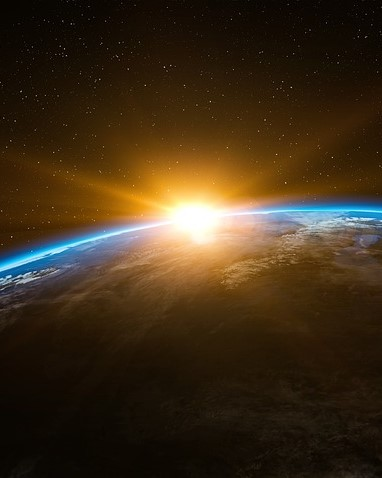
\includegraphics[width=\paperwidth,height=\paperheight]{space2}}; % original picture size was 8.08"x11.56"
\draw (current page.south) node [fill=white!30!white,fill opacity=0.6,text opacity=1,inner sep=1cm, anchor=south]{\Huge\centering\bfseries\sffamily\parbox[c][][t]{\paperwidth}{\centering \textsc{Systems Thinking, Engineering, and Analysis}\\[21pt] % Book title
{\huge \subtitle}}}; % subtitle different for main text and solution manual. renew command before \input{titlePage)
\end{tikzpicture}
\vfill
\endgroup

%%----------------------------------------------------------------------------------------
%	COPYRIGHT PAGE
\newpage
~\vfill
\thispagestyle{empty}
\noindent Copyright \copyright\ 2018 Wolter J Fabrycky\\ % Copyright notice
\noindent \textsc{Published by ACE, a Zachary D Miller company}\\ % Publisher
\noindent \textsc{\url{www.a2i2.com}}\\ % URL
\noindent Licensed under the Creative Commons Attribution-NonCommercial 3.0 Unported License (the ``License''). You may not use this file except in compliance with the License. You may obtain a copy of the License at \url{http://creativecommons.org/licenses/by-nc/3.0}. Unless required by applicable law or agreed to in writing, software distributed under the License is distributed on an \textsc{``as is'' basis, without warranties or conditions of any kind}, either express or implied. See the License for the specific language governing permissions and limitations under the License.\\ % License information
\noindent \textit{First electronic publication, 2018} % Printing/edition date

%%----------------------------------------------------------------------------------------
%	TABLE OF CONTENTS
%\usechapterimagefalse % If you don't want to include a chapter image, use this to toggle images off - it can be enabled later with \usechapterimagetrue
\chapterimage{chain.jpg} % Table of contents heading image
\pagestyle{empty} % No headers
\tableofcontents % Print the table of contents itself
% undesirable as an e-book
%\cleardoublepage % Forces the first chapter to start on an odd page so it's on the right
\pagestyle{fancy} % Print headers again

%%----------------------------------------------------------------------------------------
%	MAIN CONTENT
\part{Systems and Systems Thinking}

  \chapterimage{purpleLeaf.jpg}
  \chapter{The World in Which We Live}
    \section{Sectors Comprising Our World}
      \label{sec:sectors-comprising-our}\index{Sectors Comprising Our World}% placeholder for Sectors Comprising Our World
    \section{General Understanding of Systems}
    \section{Technology and Engineered Systems}
    \section{Transitioning Into the Systems Age}
    \section{The Evolution of Systems Thinking}
    \section{STEA as STEM for Grownups}
    \section{Summary and Extensions: insert nameref}	% \nameref{ch:the-world-in}
      \index{Summary and Extensions}% placeholder for Systems and Systems Thinking
    \section{Problems and Exercises: insert nameref}%% SEA CHAPTER 1 - SYSTEM SCIENCE AND ENGINEERING
% SEA Question Location in \label{sea-Chapter#-Problem#}
% ANSWERS NEED UPDATING
\begin{exercises}
    \begin{exercise}
    \label{sea-1-26}
        Describe how systems thinking differs from systems engineering.
        % What benefits could result from improving systems thinking in society?
    \end{exercise}
    \begin{solution}
        Human society is characterized by its culture. Each human culture manifests itself through the medium of technology. It takes more than a single step for society to transition from the past, to present and future technology states. A common societal response is often to make the transition and then to adopt a static pattern of behavior. A better response would be to continuously seek new but well-thought-out possibilities for advancement. Improvement in technological literacy embracing systems thinking should increase the population of individuals capable of participating in this desirable endeavor. \textbf{Reference:}
    \end{solution}
    
    \begin{exercise}
    \label{sea-1-1}
        For a system with which you are familiar, justify why it is a system according to the definition in \Cref{sec:sectors-comprising-our}.
        % Pick a system with which you are familiar and verify that it is indeed a system per the system definition given at the beginning of Section 1.1.
    \end{exercise}
    \begin{solution}
        A river system (Mississippi) is an assemblage of a watershed, tributaries, and river banks that conveys water from the continental U.S. to the Gulf of Mexico. A municipal transportation system (Chicago) is an assemblage of trains, buses, subways, etc. that transports people among many city locations. A system of organization and management (Matrix) is based on a morphology and procedure, coordinating both line and support functions. An automobile manufacturer is a combination of factories, organizations, dealerships, etc., that delivers automobiles and related support services. A home is an assemblage of land, structure, utilities, furnishings, and people that provides a supportive place to live for one or more families. \textbf{Reference:}
    \end{solution}
    
    \begin{exercise} 
    \label{sea-1-2}
        Describe the components, attributes, and relationships in the system you used in Problem \ref{sea-1-1}.
        % Name and identify the components, attributes, and relationships in the system you picked in Question 1.
    \end{exercise}
    \begin{solution}
        The major components of a home are listed in Answer 1 above. Attributes include acreage, terrain, square footage, utility capacities, styles of decorating and furnishing, personalities, and philosophies. Relationships include layout, allocation of space to people, and approaches to living together. \textbf{Reference:}
    \end{solution}
    
    \begin{exercise}
    \label{sea-1-3}
        Name any system which includes a material that transforms over the system's life cycle and identify its structural components, operating components, and flow components.
        % Pick a system that alters material and identify its structural components, operating components, and flow components.
    \end{exercise}
    \begin{solution}
        A chemica1 processing plant is composed of structural components (building, tanks, piping), operating components (pumps, valves, controls), and flow components (chemical constituents, energy, information). \textbf{Reference:}
    \end{solution}
    
    \begin{exercise} 
    \label{sea-1-4_5}
        Name any complex system and
        \begin{enumerate}[label=\alph*)]
            \item Define the hierarchy related to the system.
            \item Define the system boundaries.
        \end{enumerate}
        % Select a complex system and discuss it in terms of the hierarchy of systems.
        % Select a complex system and identify some different ways of establishing its boundaries.
    \end{exercise}
    \begin{solution}
        A dam system can be considered a complex system.
        \begin{enumerate}[label=\alph*)]
            \item todo
            \item The boundaries of a dam system can be limited to the physical dam. Alternatively, the human-modified river system, which now has a lake, can be considered a part of the dam system. The related road system, for which the dam now provides a bridge over the river, can be included. The region’s tourism service system, for which the dam system now provides an array of additional services, can be included. \textbf{Reference:}
        \end{enumerate}
    \end{solution}
    
    \begin{exercise} 
    \label{sea-1-6_7_8}
        Identify and contrast
        \begin{enumerate}[label=\alph*)]
            \item Physical versus conceptual systems.
            \item Static versus dynamic systems.
            \item Closed versus open systems.
        \end{enumerate}
        % Identify and contrast a physical and conceptual system.
        % Identify and contrast a static and a dynamic system.
        % Identify and contrast a closed and an open system.
    \end{exercise}
    \begin{solution}
        \begin{enumerate}[label=\alph*)]
            \item A physical system such as a watershed has components which manifest themselves in space and time, whereas a conceptual system such as a work breakdown structure has no physical manifestations. It is only a plan for action. Reference: Section 1.2.2 (pages 6-7).
            \item A static system such as a highway system may be contrasted with an airline system, which is a dynamic system. In the former, structure exists without activity whereas in the latter, structural components are combined with the activities of aircraft being loaded and unloaded, aircraft in flight, and controls which govern the entire operation. Reference: Section 1.2.3 (page 7).
            \item A cannon is an example of a closed system. When a cannon is fired, a one–to–one correspondence exists between the initial and final states. However, the defense contractor’s design and manufacturing organization that produced the cannon and associated projectile is an open system, with a dynamic interaction of system components. These system components must be reconfigured and adapted to cope with changing requirements. \textbf{Reference:}
        \end{enumerate}
    \end{solution}
    
    \begin{exercise} 
    \label{sea-1-15}
        For any system of the following types, name any system property
        \begin{enumerate}[label=\alph*)]
            \item Dynamic system.
            \item Steady-state system.
        \end{enumerate}
        % Give an example of a random dynamic system property and of a steady state dynamic system property.
    \end{exercise}
    \begin{solution}
        \textbf{Reference:}
    \end{solution}
    
    \begin{exercise} 
    \label{sea-1-9}
        For each of the following systems, define a unique system and describe it in terms of components, attributes, and relationships
        \begin{enumerate}[label=\alph*)]
            \item Natural system.
            \item Human-made system.
            \item Human-modified system.
        \end{enumerate}
        % Pick a natural system and describe it in terms of components, attributes, and relationships; repeat for a human-made system; repeat for a human-modified system.
    \end{exercise}
    \begin{solution}
        \begin{enumerate}[label=\alph*)]
            \item A watershed is a natural system made up of objects or components such as land, vegetation, and the watercourse; attributes such as the soil type, timber species, and the river width; and relationships such as the distribution of the attributes over the terrain. 
            \item A chemical processing plant is a human–made system with components described in Answer 3 above, attributes such as tank volume and pipe diameter, and relationships such as the flow rates and the yield of final product per energy unit utilized.
            \item A person with a pacemaker is a human-modified system with components of body parts and pacemaker parts, attributes such as body mass, diseases, attitudes, battery, controller, and electrodes, and relationships such as implantation location, rhythm, and signal strength. \textbf{Reference:}
        \end{enumerate}
    \end{solution}
    
    \begin{exercise} 
    \label{sea-1-10_11_12}
        For any Human-made system (including the system from \ref{sea-1-9})
        \begin{enumerate}[label=\alph*)]
            \item Identify the system's purpose(s) and potential metrics to present its value.
            \item Describe the system's state at any arbitrary time during operation, at least one system behavior, and an overview of the system's process.
            \item Name any two related components of the system, define the purpose of each component as it relates to the other, and the necessary attributes of the component pair such that they contribute to the purpose(s) of the entire system.
        \end{enumerate}
        % Identify the purpose(s) of the above human-made system and name some possible measures of worth.
        % For the above human-made system, describe its state at some point in time, describe one of its behaviors, and summarize its process.
        % For the above human-made system, name two components that have a relationship, identify what need each component fills for the other component, and describe how the attributes of these two components must be engineered so that the pair functions together effectively in contributing to the system’s purpose(s).
    \end{exercise}
    \begin{solution}
        \begin{enumerate}[label=\alph*)]
            \item The purposes of a chemical processing plant in a market economy are to produce one or more chemical products and possibly byproducts that can be sold at a profit while fulfilling obligations to stakeholders and the public. Measures of worth include production cost per unit volume, product quality, flexibility of product mix, benefits to stakeholders, and compatibility with society. \textbf{Reference:}
            \item During startup the state of a chemical processing plant is that pipes and vessels are filled to a certain location and empty after that location; pumps for vessels being filled are running and valves are open while other pumps are not running and valves are closed. A behavior is that when a vessel is filled, the control system turns off the pump (in a batch system) or reduces its speed (in a continuous system) and activates the next step in the process. The process is to start up, achieve the designated operational speed for each subsystem, continuously monitor the production results and make needed adjustments, and eventually shut down and clean out. \textbf{Reference:}
            \item A pump and the tank it fills have a relationship. The pump provides the material that the tank needs, while the tank provides a location where the pump can store the material it needs to deliver. The attributes of the pump must be engineered so that it can reliably move the material(s) the tank needs at an adequate rate for any given speed of overall system operation. The attributes of the tank must be engineered so that it can store the quantities of material the pump must deliver without corrosion or contamination. Thus the downstream components have the material they need to fulfill the plant’s production purpose without problems of quality or pollution. \textbf{Reference:} 
        \end{enumerate}
    \end{solution}
    
    \begin{exercise} 
    \label{sea-1-14}
        For any Human-modified system (including the system from \ref{sea-1-9}), name some positive and negative impact(s) of the modification to the natural system.
        % For a human-modified system, identify some of the ways in which the modified natural system could be degraded and some of the ways in which it could be improved.
    \end{exercise}
    \begin{solution}
        Human introduction of plant or animal species into regions where they do not naturally occur can provide the benefits of those species in the new regions, but the new species may become excessively dominant in those regions due to lack of natural enemies, crowding out or harming beneficial native species. \textbf{Reference:}
    \end{solution}
    
    \begin{exercise} 
    \label{sea-1-13}
        Give examples of each of the following
        \begin{enumerate}[label=\alph*)]
            \item First-order relationship.
            \item Second-order relationship.
            \item Redundance.
        \end{enumerate}
        % Give an example of a first-order relationship, a second-order relationship, and redundance.
    \end{exercise}
    \begin{solution}
        \begin{enumerate}[label=\alph*)]
            \item In a computer system, the power supply and system board have a first-order relationship because the system board must receive the reduced voltage produced by the power supply in order to function, and the power supply would be useless if there were no system board to perform and coordinate the computer functions. 
            \item The system board has a second-order relationship with a math coprocessor, or a video processor, or with video memory. The system board could perform the functions of these additional components, but the added components relieve the system board’s workload, thereby improving its performance.
            \item  A second power supply or a mirror image hard disk drive provide redundance, ensuring that the system board can continue receiving electrical power and the data storage function, thereby helping to assure continuation of the computer system function. \textbf{Reference:}
        \end{enumerate}
    \end{solution}
    
    \begin{exercise} 
    \label{sea-1-16}
        Name any system that operates at equilibrium and another system that degrades over time.
        % Give an example of a system that reaches equilibrium and of a system that disintegrates over time.
    \end{exercise}
    \begin{solution}
        A forest reaches equilibrium. A tree is in equilibrium until it dies, and then it disintegrates. \textbf{Reference:}
    \end{solution}
    
    \begin{exercise} 
    \label{sea-1-17}
        The United States government, for example, can be divided and described as three individual entities of the executive, legislative, and judicial branches. Create an argument for why a government of this structure should either be considered a single system or three systems.
        % Is a government with executive, legislative, and judicial branches three systems or a single system? Why?
    \end{exercise}
    \begin{solution}
        The government described is a single system because the branches thereof are functionally related. \textbf{Reference:}
    \end{solution}
    
    \begin{exercise} 
    \label{sea-1-19}
        Give any example of cybernetics and define why the example is appropriate.
        % Explain cybernetics by using an example of your choice.
    \end{exercise}
    \begin{solution}
        Cybernetics may be described and explained by considering the early mechanical version of a governor to control the revolutions per minute (RPM) of an engine. Centrifugal force, acting through a weight mechanism on the flywheel, is used to sense RPM. The outward movement of the weight against a spring acts through a link to decrease the throttle setting, thus reducing engine speed. \textbf{Reference:}
    \end{solution}
    
    \begin{exercise} 
    \label{sea-1-21}
        Do all systems at higher levels of Boulding's Hierarchy necessarily incorporate the lower levels of the hierarchy? If not, provide a specific system example.
        % Select a system at one of the higher levels in Boulding’s hierarchy and describe if it does or does not incorporate the lower levels.
    \end{exercise}
    \begin{solution}
        \textbf{Reference:}
    \end{solution}
    
    \begin{exercise} 
    \label{sea-1-22}
        Describe a novel system that may be necessary for society 50 to 100 years in the future and
        \begin{enumerate}[label=\alph*)]
            \item Define the system requirements.
            \item Define the system objectives.
        \end{enumerate}
        % Identify a societal need, define the requirements of a system that would fill that need, and define the objective(s) of that system.
    \end{exercise}
    \begin{solution}
        Efficient transportation system to the Moon and/or Mars. \textbf{Reference:}
    \end{solution}
    
    \begin{exercise} 
    \label{sea-1-25}
        For the system described in Question \ref{sea-1-22}
        \begin{enumerate}[label=\alph*)]
            \item Identify factors which led to the need for a new system.
            \item Identify other societal factors which may evolve in parallel and lead to other changes or innovations.
        \end{enumerate}
        % Name some of the factors driving technological advancement and change.
    \end{exercise}
    \begin{solution}
        \begin{enumerate}[label=\alph*)]
            \item Factors driving technological change include attempts to respond to unmet current needs and attempts to perform ongoing activities in a more efficient and effective manner, as well as social factors, political objectives, ecological concerns, and the desire for environmental sustainability. \textbf{Reference:}
            \item todo
        \end{enumerate}
    \end{solution}
    
    \begin{exercise} 
    \label{sea-1-23}
        Compare and contrast systemology and synthesis.
        % What are the similarities of systemology and synthesis?
    \end{exercise}
    \begin{solution}
        Both systemology and synthesis produce systems. Systemology produces a system of processes by which systems are brought into being and carried through the life cycle. Synthesis produces any kind of system. Synthesis is a part of systemology and also a product of systemology. \textbf{Reference:}
    \end{solution}
    
    \begin{exercise} 
    \label{sea-1-24}
        Classify a technical system.
        % What difficulty is encountered in attempting to classify technical systems?
    \end{exercise}
    \begin{solution}
        The phrase “technical system” is used to represent all types of human–made artifacts, including engineered products and processes. Classifying a technical system is generally difficult, because a technical system derives its inputs from several disciplines or fields which may be very different from one another. \textbf{Reference:}
    \end{solution}
    
    \begin{exercise} 
    \label{sea-1-27}
        Compare and contrast the attributes of the Machine (Industrial) Age and the Systems Age.
        % Identify the attributes of the Machine or Industrial Age and the Systems Age.
    \end{exercise}
    \begin{solution}
        Attributes of the Machine Age are determinism, reductionism, physical, cause and effect, and closed system thinking. The Systems Age has attributes of open systems thinking, expansionism, human–machine interfacing, automation, optimization, and goal orientation. \textbf{Reference:}
    \end{solution}
    
    \begin{exercise} 
    \label{sea-1-28}
        Identify key differences between synthetic and analytical thinking. Is one method of thinking always preferable? Why or why not?
        % Explain the difference between analytic and synthetic thinking.
    \end{exercise}
    \begin{solution}
        Analytic thinking seeks to explain the whole based on explanations of its parts. Synthetic thinking explains something in terms of its role in a larger context. \textbf{Reference:}
    \end{solution}
    
    \begin{exercise} 
    \label{sea-1-29}
        What challenges make the Systems Age unique from other periods of human evolution?
        % What are the special engineering requirements and challenges in the Systems Age?
    \end{exercise}
    \begin{solution}
        The special engineering requirements of the Systems Age are those which pertain to integration, synthesis, simulation, economic analysis, and environmental concerns, along with the necessity to bring the classical engineering disciplines to bear on the system under development through collaboration. \textbf{Reference:}
    \end{solution}
    
    \begin{exercise} 
    \label{sea-1-30}
        Compare and contrast systems engineering with other engineering disciplines.
        % What are the differences (and similarities) between systems engineering and the traditional engineering disciplines?
    \end{exercise}
    \begin{solution}
        Both systems engineering and the traditional engineering disciplines deal with technology and technical (human-made) entities. The focus of traditional engineering is on technical design of the entities in human-made systems, whereas systems engineering concentrates on what the entities are intended to do (functional design) before determining what the entities are. Traditional engineering focuses on technical performance measures, whereas systems engineering considers all requirements of the client, system owner, and/or the user group, as well as the effects on related systems. Traditional engineering focuses on designing products for their operational uses, whereas systems engineering considers all the life cycles of the systems that include its products. Traditional engineering tends to proceed from the bottom-up, whereas systems engineering favors a top-down approach. Traditional engineering favors analytic thinking while systems engineering favors synthetic thinking. Traditional engineering applies the skills of particular engineering disciplines to problems, whereas systems engineering defines problems before determining what disciplines are needed. Systems engineering provides methodologies that facilitate effective teamwork among not only the traditional engineering disciplines, but also among other technical as well as social disciplines. \textbf{Reference:}
    \end{solution}
    
    \begin{exercise} 
    \label{sea-1-32}
        Identify a system which required an interdisciplinary approach to develop \textit{or} to implement. What disciplines were required and why?
        % Give an example of a problem requiring an interdisciplinary approach and identify the needed disciplines.
    \end{exercise}
    \begin{solution}
        The problem of predicting the availability and amount of oil and natural gas from a certain geological region, which might be available to refineries and power plants in another region in future time periods, requires the disciplines of geology, petroleum engineering, regional planning, civil engineering, ecological science, transportation engineering, and economics. The validity of the prediction depends largely upon the proper utilization and interpretation of findings by the relevant disciplines and their domains of inquiry. \textbf{Reference:}
    \end{solution}
    
    \begin{exercise} 
    \label{sea-1-33}
        Identify an interdiscipline and the disciplines from which it was derived.
        % Name an interdiscipline and identify the disciplines from which it was drawn.
    \end{exercise}
    \begin{solution}
        Systems engineering is an interdiscipline (sometimes called a multidiscipline or transdiscipline) drawn mainly from the engineering disciplines, but also from mathematics, operations research, systemology, project management, and increasingly, other fields. \textbf{Reference:}
    \end{solution}
    
    \begin{exercise} 
    \label{sea-1-35_36_38}
        For the following organizations, summarize their mission statements
        \begin{enumerate}[label=\alph*)]
            \item \href{http://isss.org/}{International Society for the Systems Sciences}
            \item \href{https://www.incose.org/}{International Council on Systems Engineering}
            \item \href{https://omegalpha.org/}{Omega Alpha Association}
        \end{enumerate}
        % Go to the website for ISSS given in Section 1.7 and summarize the goal of the society.
        % Go to the website for INCOSE given in Section 1.7 and summarize the goals of the council.
        % Go to the website for OAA and compare this honor society with one that you are familiar with.
    \end{exercise}
    \begin{solution}
        \begin{enumerate}[label=\alph*)]
            \item Independent exercise. Visit http://isss.org/
            \item Independent exercise. Visit https://www.incose.org/
            \item Independent exercise. Visit https://omegalpha.org/
        \end{enumerate}
    \end{solution}
    
    \begin{exercise} 
    \label{sea-1-37}
        Explain how the goals of ISSS and INCOSE differ.
        % Contrast the goals of ISSS and INCOSE as given in Section 1.7 or on the web.
    \end{exercise}
    \begin{solution}
        Independent exercise. Refer to the solution of \ref{sea-1-35_36_38}.
    \end{solution}
\end{exercises}
% SKIPPED
% sea-1-18 Identify a system-of-systems whose analysis could yield insights not available by separately analyzing the individual systems of which it is composed.
% sea-1-20 Give a system example at any five of the levels in Boulding’s hierarchy.
% sea-1-31 Given the recommendations in Educating the Engineer of 2020, what should be added to the curriculum with which you are familiar?
% sea-1-34 Write your own (preferred) definition of systems engineering.
    
  \chapterimage{wireFrame.jpg}
  \chapter{Scientific Thinking and Knowledge}
    \section{Human Curiosity and Inquiry}
    \section{Human Activity and Praxeology}
    \section{Scientific Thinking in Antiquity}
    \section{Contemporary Scientific Thinking}
    \section{Science and Systems Science}
	\section{Valuing Faith-Based Thinking}
	\section{Summary and Extensions: insert nameref}
	   \index{Summary and Extensions}% placeholder for Systems and Systems Thinking
	\section{Problems and Exercises: insert nameref}%% SEA CHAPTER 2 - BRINGING SYSTEMS INTO BEING
% SEA Question Location in \label{sea-Chapter#-Problem#}
% ANSWERS NEED UPDATING
\begin{exercises}
    \begin{exercise}
    \label{sea-2-1}
        Identify at least two characteristics that distinguish natural systems from those that are human-made or human-modified.
        % What are some of the characteristics of a human-made or engineered system that distinguish it from a natural system?
    \end{exercise}
    \begin{solution}
        A human–made or engineered system comes into being by purpose-driven human action. It is distinguished from the natural world by characteristics imparted by its human originator, innovator, or designer. The human–made system is made up of elements (materials) extracted from the natural world and it is then embedded therein. Human–made systems may or may not meet human needs in a satisfactory manner. \textbf{Reference:}
    \end{solution}
    
    \begin{exercise}
    \label{sea-2-2}
        Identify at least two possible interfaces between the natural and human worlds for the creation of any arbitrary system.
        % Describe some of the interfaces between the natural world and the human-made world as they pertain to the process of bringing systems/products into being.
    \end{exercise}
    \begin{solution}
        Interfaces between the human–made and the natural world arise from human–made products, systems, and structures for the use of people. An example interface is a system of pipes, pumps, and tanks bringing water from a natural system, such as a lake, or a human– made system like a reservoir, to a city. The human–made water distribution system creates an interface when it is brought into being. Interface-creating entities such as this draw upon natural resources and impact the environment during use and at the end of their useful life. \textbf{Reference:}
    \end{solution}
    
    \begin{exercise}
    \label{sea-2-3}
        Describe what distinguishes human-made from human-modified systems.
        % Identify and describe a natural system of your choice that has been human-modified and identify what distinguishs it from a human-made system.
    \end{exercise}
    \begin{solution}
        A watershed in its natural state is a natural system that receives rainfall, absorbs some rainwater, and accumulates and discharges runoff. This system becomes human-modified if a dam is constructed at a point on the watercourse. The watershed is now a humanmodified system that differs from the original system. Some differences are the new capacity for water storage, a change in the rate of runoff, and some change in the pattern of water absorption into the soil. A change will also occur in the distribution and density of vegetation in the watershed. \textbf{Reference:}
    \end{solution}
    
    \begin{exercise}
    \label{sea-2-5_6}
        Based on the textbook descriptions in ???, identify a system for the following system types and justify your answer based on the system product(s).
        \begin{enumerate}[label=\alph*)]
            \item Single-entity product system.
            \item Multiple-entity product system.
        \end{enumerate}
        % Put a face on the generic single-entity product system of Section 2.1.2 by picking a real structure or service with which you are familiar. Then, rewrite the textbook description based on the characteristics of the entity you picked.
        % Put a face on the generic multiple-entity population system of Section 2.1.2 by picking real equipment with which you are familiar. Then, rewrite the textbook description based on the characteristics of the equipment you picked.
    \end{exercise}
    \begin{solution}
        \begin{enumerate}[label=\alph*)]
            \item todo
            \item todo
        \end{enumerate}
    \end{solution}
    
    \begin{exercise}
    \label{sea-2-7_8}
        Choose any consumer item and identify the producer. Then
        \begin{enumerate}[label=\alph*)]
            \item Identify at least three things that are employed or consumed by the producer to create the consumer item.
            \item Identify any enabling system which is employed by the producer to create the consumer item.
            \item Must an enabling system and a product of that system be engineered jointly? Why or why not?
        \end{enumerate}
        % Pick a consumer good and name the producer good(s) that need to be employed to bring this consumer good to market.
        % Pick a product, describe the enabling system that is required to bring it into being, and explain the importance of engineering the system and product together.
    \end{exercise}
    \begin{solution}
        \begin{enumerate}[label=\alph*)]
            \item todo
            \item todo
            \item todo
        \end{enumerate}
    \end{solution}
    
    \begin{exercise} 
    \label{sea-2-9}
        Identify at least four factors which determine a product's competitiveness. Is product competitiveness important? Why or why not?
        % What are some of the essential factors in engineering for product competitiveness? Why is product competitiveness important?
    \end{exercise}
    \begin{solution}
        The quality, price, ergonomics, and lifetime of a product would all be considered to influence the purchasing behavior of consumers, which is based on product competition. ORIGINAL: The overarching factor in engineering for product competitiveness is the requirement to meet customer expectations cost–effectively. Competitiveness is the assurance of corporate health and advancement in the global marketplace. This desideratum cannot be achieved by advertising, acquisitions, mergers, and outsourcing alone. Product competitiveness requires focus on design characteristics. Product (and system) design is now being recognized by forward-looking enterprises as an underutilized strategic weapon. \textbf{Reference:}
    \end{solution}
    
    \begin{exercise}
    \label{sea-2-10}
        Explain the benefits of system life-cycle thinking and why it is important.
        % What does system life-cycle thinking add to engineering as currently practiced? What are the expected benefits to be gained from this thinking?
    \end{exercise}
    \begin{solution}
        System life–cycle thinking necessitates engineering for the life cycle. This is in contrast to engineering as historically practiced, in which downstream considerations were often deferred or neglected. Life–cycle thinking can help preclude future problems if emphasis is placed on: (a) Improving methods for defining system and product requirements; (b) Addressing the total system with all its elements from a life–cycle perspective; (c) Considering the overall system hierarchy and the interactions between various levels in that hierarchy.\\
        Some of the problems that life–cycle thinking can help alleviate are: (a) The dwindling of available resources by looking ahead and considering timely substitution; (b) The erosion of the industrial base through international competition by emphasizing design–based strategies; (c) The loss of market share by providing the right product at the right price to avoid the need to downsize or merge to synchronize operations; (d) The demand for more complex products, which increases the cost of operations for the producer. \textbf{Reference:}
    \end{solution}
    
    \begin{exercise}
    \label{sea-2-11}
        For the product life-cycles displayed in Figures ???, ???, identify possible sources of feedback or communication between the different phases.
        % Various phases of the product life cycle are shown in Figure 2.1 and expanded in Figure 2.2. Describe some of the interfaces and interactions between the life cycles of the system and the product life cycle.
    \end{exercise}
    \begin{solution}
        The first life cycle involves technological activity beginning with need identification and revolves around product design and development. Consideration is then given to the production or construction of the product or structure. This is depicted in the second life cycle which involves bringing a manufacturing or construction capability into being. The third life cycle concerns the maintenance and logistic support needed to service the product during use and to support the manufacturing capability. Finally, the fourth life cycle addresses the phase–out and disposal of system and product elements and materials. \textbf{Reference:}\\
        The major functions of the system engineering process during conceptual design are the establishment of performance parameters, operational requirements, support policies, and the development of the system specification. As one proceeds through design and development, the functions are primarily system dependent, and may include functional analyses and allocations to identify the major operational and maintenance support functions that the system is to perform. Criteria for system design are established by evaluating different (alternative) design approaches through the accomplishment of system/cost effectiveness analyses and trade–off studies, the conduct of formal design reviews, and preparing system development, process, and material specifications. The production and/or construction phase may entail technical endeavors such as the design of facilities for product fabrication, assembly, and test functions; design of manufacturing processes; selection of materials; and the determination of inventory needs. The major functions during system use and life–cycle support can involve providing engineering assistance in the initial deployment, installation, and checkout of the system in preparation for operational use; providing field service or customer service; and providing support for phase–out and disposal of the system and its product for the subsequent reclamation and recycling of reclaimable components.
    \end{solution}
    
    \begin{exercise}
    \label{sea-2-12}
        Pretend that you are developing a product. How do you convince your peer(s) that the best approach is to \say{design for the life cycle}?
        % What is the full meaning of the phrase “designing for the life cycle”?
    \end{exercise}
    \begin{solution}
        Designing for the life cycle means thinking about the end before the beginning. It questions every design decision on the basis of anticipated downstream impacts. Design for the life cycle is enabled by application of systems engineering defined as an interdisciplinary approach to derive, evolve, and verify a life–cycle balanced system solution which satisfies customer expectations and meets stakeholder expectations. It promotes a top– down, integrated life–cycle approach to bringing a system into being, embracing all of the phases exhibited in ???. \textbf{Reference:}
    \end{solution}
    
    \begin{exercise}
    \label{sea-2-14} 
        Identify one benefit and one consequence of the following design models
        \begin{enumerate}[label=\alph*)]
            \item Waterfall model.
            \item Spiral model.
            \item V-model.
        \end{enumerate}
        % As best you can, identify life-cycle activities that occur in the waterfall model, the spiral model, and the “vee” model. Of these models, pick the one you prefer and explain why.
    \end{exercise}
    \begin{solution}
        \begin{enumerate}[label=\alph*)]
            \item Independent exercise.
            \item Independent exercise.
            \item Independent exercise.
        \end{enumerate}
    \end{solution}
    
    \begin{exercise}
    \label{sea-2-14_part2}
        Of the models described in \Cref{sea-2-14}, do you have a personal preference? Is any one model always the most appropriate? Why or why not?
        % As best you can, identify life-cycle activities that occur in the waterfall model, the spiral model, and the “vee” model. Of these models, pick the one you prefer and explain why.
    \end{exercise}
    \begin{solution}
        \begin{enumerate}[label=\alph*)]
            \item Independent exercise.
        \end{enumerate}
    \end{solution}
    
    \begin{exercise}
    \label{sea-2-15_16}
        Select a design situation of your choice.
        \begin{enumerate}[label=\alph*)]
            \item What are the requirements of the system?
            \item Describe the steps for identifying appropriate technical performance measures.
            \item Describe the relationship between the system requirements and its technical performance measures.
            \item What happens when the technical performance measures disagree with the system requirements?
        \end{enumerate}
        % Design considerations are the first step on the way to deriving technical performance measures. Outline all of the steps, emphasizing the design-dependent parameter concept.
        % How are requirements related to technical performance measures? What is the remedy when requirements and TPMs are not in agreement?
    \end{exercise}
    \begin{solution}
        \begin{enumerate}[label=\alph*)]
            \item After the need has been identified, it should be translated into system operational requirements. In determining system requirements, the engineering design team needs to know what the system is to accomplish, when the system will be needed, how the system is to be utilized, what effectiveness requirements the system should meet, how the system is to be supported during use, and what the requirements are for phase–out and disposal.
            \item TPMs identify the degree to which the proposed design is likely to meet customer expectations. Many parameters may be of importance in a specific design application and most of these are design–dependent. These are appropriately called design–dependent parameters (DDPs). 
            \item Requirements are the driving force for identifying those design considerations that must be measured and expressed as TPMs. TPMs are specific estimated and/or predicted values for DDPs and they may or may not match required values. 
            \item When requirements and TPMs are not in agreement, the system design endeavor must be continued by altering those factors and/or design characteristics upon which design values inherently depend; i.e., DDPs. Alternatively, the customer may be made aware of the discrepancy and be given the opportunity to modify initially stated requirements.
        \end{enumerate}
    \end{solution}
    
    \begin{exercise}
    \label{sea-2-18_20}
        Select a design situation of your choice and refer to figure ??? for the following questions.
        \begin{enumerate}[label=\alph*)]
            \item Identify a top-level requirement and decompose it appropriately.
            \item Identify a lowest-level requirement and explain its relevance for all higher levels.
        \end{enumerate}
        % Pick a top-level requirement and decompose it in accordance with the structure shown in Figure 2.7.
        % Pick up on a design consideration at the lowest level in Figure 2.8. Discuss its position and impact on each of the next higher levels.
    \end{exercise}
    \begin{solution}
        \begin{enumerate}[label=\alph*)]
            \item Independent exercise.
            \item Independent exercise.
        \end{enumerate}
    \end{solution}
    
    \begin{exercise}
    \label{sea-2-22}
        Identify at least three domain manifestations of systems engineering.
        % Identify some of the engineering domain manifestations of systems engineering.
    \end{exercise}
    \begin{solution}
        Formal engineering domain manifestations of systems engineering that are offered as academic degrees are biological systems engineering, computer systems engineering, industrial systems engineering, manufacturing systems engineering, and others. Informal domains exist with employment opportunities in aerospace systems engineering, armament systems engineering, network systems engineering, information systems engineering, health systems engineering, service systems engineering, and many others. \\
        Systems engineering utilizes appropriately applied technological inputs from various engineering disciplines together with management principles in a synergistic manner to create new systems. Traditional engineering domains tend to focus on the bottom–up approach in designing new systems, whereas systems engineering uses the top–down approach. Unlike the traditional disciplines, it adopts a life–cycle approach in the design of new systems. \textbf{Reference:}
    \end{solution}
    
    \begin{exercise}
    \label{sea-2-23}
        Identify at least three obstructions which hinder or prevent the application of systems engineering.
        % What are some of the impediments to the implementation of systems engineering?
    \end{exercise}
    \begin{solution}
        Some organizational impediments to the implementation of systems engineering include: (a) the dominance of disciplines over interdisciplines, (b) a tendency to organize SE in the same manner as the traditional engineering disciplines, (c) an excessive focus on analysis at the expense of synthesis and process, (d) difficulty in integrating the appropriate discipline contributions with the relevant system elements, (e) the lack of sufficient communication, especially where system contributors are geographically dispersed, (f) deficiencies in balancing technologies and tools with planning and management of the activities required to accomplish objectives, (g) an ineffective general organizational environment to enable the systems engineering function to truly impact design and system development. Other impediments related to the above include (a) the lack of a good understanding of customer needs and definition of the system requirements, (b) ignorance of the fact that the majority of the projected life-cycle cost for a given system is committed because of engineering design and management decisions made during the early stages of conceptual and preliminary design, (c) the lack of a disciplined top–down “systems approach” in meeting desired objectives, (d) system requirements defined from a short term perspective and, (e) lack of good planning early, and the lack of subsequent definition and allocation of requirements in a complete and disciplined manner. \textbf{Reference:}
    \end{solution}
    
    \begin{exercise}
    \label{sea-2-24}
        Why is systems thinking and engineering beneficial?
        % What are some of the benefits that may result from the utilization of systems thinking and engineering?
    \end{exercise}
    \begin{solution}
        Some of benefits that accrue from the application of the concepts and principles of systems engineering are: (a) Tailoring involving the modification of engineering activities applied in each phase of the product or system life cycle to adapt them to the particular product or system being brought into being. Its importance lies in that the proper amount of engineering effort must be applied to each phase of the system being developed, and it must be tailored accordingly; (b) Reduction in the life–cycle cost of the system. Often it is perceived that the implementation of systems engineering will increase the cost of the system acquisition. This is misconception since there might be more steps to perform during the early (conceptual and preliminary) system design phases, but this could reduce the requirements in the integration, test and evaluation efforts later in the detail design and development phase; (c) More visibility and a reduction of risks associated with the design decision making process, with a consequent increase in the potential for greater customer satisfaction; (d) promotion of a top–down integrated life–cycle approach for bringing a system into being. \\
        The benefit of systems engineering is needed when the engineering specialists in one of more of the conventional engineering areas may not be sufficiently experienced or capable to ensure that all elements of the system are orchestrated in a proper and timely manner. \textbf{Reference:}
    \end{solution}
\end{exercises}
% SKIPPED
% sea-2-4 Describe the product or prime equipment as a component of the system; provide an explanation of the functions provided by each entity.
% sea-2-13 Select a system of your choice and describe the applicable life-cycle phases and activities, tailoring your description to that system.
% sea-2-17 Pick a design situation of your choice and itemize the multiple criteria that should be addressed.
% sea-2-19 Candidate systems result from design synthesis and become the object of design analysis and evaluation. Explain.
% sea-2-21 Take synthesis, analysis, and evaluation as depicted in Figure 2.9 and then classify each activity exhibited by application of elements in the ten-block morphology of Figure 2.10.
% sea-2-25 Go to the INCOSE web site and find the page about the Systems Engineering Journal. Pick an article that touches upon a topic in this chapter and relate it thereto using no more than one paragraph.
% sea-2-26 Go to the INCOSE web site and identify one individual from the Fellows group who most closely matches your own interest in systems engineering. Say why you would like to meet this person.
  
  \chapterimage{leaf-bottom.jpg}
  \chapter{Organizing Human Activity Systems}
    \section{Humans and Human Nature}
    \section{Humankind's Most Important Innovation}
    \section{An Organization Concept by Barnard}
    \section{Enterprises and Enterprise Systems}
    \section{Government and Governance}
    \section{Systems Engineering and Management}
    \section{Summary and Extensions: insert nameref}
       \index{Summary and Extensions}% placeholder for Systems and Systems Thinking
    \section{Problems and Exercises: insert nameref}%% SEA CHAPTER 3 - CONCEPTUAL SYSTEM DESIGN
% SEA Question Location in \label{sea-Chapter#-Problem#}
% NEEDS UPDATING
\begin{exercises}
    \begin{exercise}
    \label{sea-3-1}
        In accomplishing a needs analysis in response to a given deficiency,what type of information would you include? Describe the process that you would use in developing the necessary information.
    \end{exercise}
    \begin{solution}
    \end{solution}
    
    \begin{exercise}
    \label{sea-3-2}
        What is the purpose of the feasibility analysis? What considerations should be addressed in the completion of such an analysis?
    \end{exercise}
    \begin{solution}
    \end{solution}
    
    \begin{exercise}
    \label{sea-3-3}
        Through a review of the literature, describe the QFD approach and how it could be applied in helping to define the requirements for a given system design.
    \end{exercise}
    \begin{solution}
    \end{solution}
    
    \begin{exercise}
    \label{sea-3-4}
        Why is the definition of system operational requirements important? What type of information is included?
    \end{exercise}
    \begin{solution}
    \end{solution}
    
    \begin{exercise}
    \label{sea-3-5}
        What specific challenges exist in defining the operational requirements for a system-of-systems (SOS) configuration? What is meant by interoperability? Provide an example.
    \end{exercise}
    \begin{solution}
    \end{solution}
    
    \begin{exercise}
    \label{sea-3-6}
        hy is it important to define specific mission scenarios (or operational profiles) within the context of the system operational requirements?
    \end{exercise}
    \begin{solution}
    \end{solution}
    
    \begin{exercise}
    \label{sea-3-7}
        What information should be included in the system maintenance concept? How is it developed (describe the steps), and at what point in the system life cycle should it be developed?
    \end{exercise}
    \begin{solution}
    \end{solution}
    
    \begin{exercise}
    \label{sea-3-8}
        How do system operational requirements influence the maintenance concept (if at all)?
    \end{exercise}
    \begin{solution}
    \end{solution}
    
    \begin{exercise}
    \label{sea-3-9}
        How does the maintenance concept affect system/product design? Give some specific examples.
    \end{exercise}
    \begin{solution}
    \end{solution}
    
    \begin{exercise}
    \label{sea-3-10}
        Select a system of your choice and develop the operational requirements for that system. Based on the results,develop the maintenance concept for the system.Construct the necessary operational and maintenance flows,identify repair policies,and apply quantitative effectiveness factors as appropriate.
    \end{exercise}
    \begin{solution}
    \end{solution}
    
    \begin{exercise}
    \label{sea-3-11}
        Refer to Figure 3.12 and assume that a similar infrastructure exists in your own community. Identify the various system capabilities (functions), illustrate (draw) an overall configuration structure (similar to that in the figure), and identify some of the critical metrics required as an input to the design of such.
    \end{exercise}
    \begin{solution}
    \end{solution}
    
    \begin{exercise}
    \label{sea-3-12}
        Refer to Figure 3.13. For a system-of-systems (SOS) configuration of your choice, describe some of the critical requirements in the design of a SOS. 
    \end{exercise}
    \begin{solution}
    \end{solution}
    
    \begin{exercise}
    \label{sea-3-13}
        In evaluating whether or not a two- or three-level maintenance concept should be specified, what factors would you consider in the evaluation process?
    \end{exercise}
    \begin{solution}
    \end{solution}
    
    \begin{exercise}
    \label{sea-3-14}
        In developing the maintenance concept, it is essential that all levels of maintenance be considered on an integrated basis. Why?
    \end{exercise}
    \begin{solution}
    \end{solution}
    
    \begin{exercise}
    \label{sea-3-15}
        Why is the development of technical performance measures (TPMs) important?
    \end{exercise}
    \begin{solution}
    \end{solution}
    
    \begin{exercise}
    \label{sea-3-16}
        Refer to Figure 3.17. Describe the steps that you would complete in developing the information included in the figure. Be specific.
    \end{exercise}
    \begin{solution}
    \end{solution}
    
    \begin{exercise}
    \label{sea-3-17}
        What is the purpose of allocation? To what depth in the system hierarchical structure should allocation be accomplished? How does it impact system design (if at all)?
    \end{exercise}
    \begin{solution}
    \end{solution}
    
    \begin{exercise}
    \label{sea-3-18}
        What is meant by functional analysis? When in the system life cycle is it accomplished? What purpose does it serve? Identify some of the benefits derived. Can a functional analysis be accomplished for any system? Can a functional analysis be accomplished for a system-of-systems (SOS) configuration?
    \end{exercise}
    \begin{solution}
    \end{solution}
    
    \begin{exercise}
    \label{sea-3-19}
        What is meant by a common function in the functional analysis? How are common functions determined? 
    \end{exercise}
    \begin{solution}
    \end{solution}
    
    \begin{exercise}
    \label{sea-3-20}
        How does the functional analysis lead into the definition of specific resource requirements in the form of hardware, software, people, data, facilities, and so on? Briefly describe the steps in the process, and include an example. What is the purpose of the block numbering shown in Figures 3.20, 3.21, and 3.22?
    \end{exercise}
    \begin{solution}
    \end{solution}
    
    \begin{exercise}
    \label{sea-3-21}
        What is the purpose of allocation? To what depth in the system hierarchical structure should allocation be accomplished? How does it impact system design (if at all)? How can allocation be applied for a SOS configuration (if at all)? 
    \end{exercise}
    \begin{solution}
    \end{solution}
    
    \begin{exercise}
    \label{sea-3-22}
        In conceptual design, there are a number of different requirements for predicting or estimating various system metrics. What approach (steps) would you apply in accomplishing such?
    \end{exercise}
    \begin{solution}
    \end{solution}
    
    \begin{exercise}
    \label{sea-3-23}
        What is the purpose of the formal design review? What are some of the benefits derived from the conduct of design reviews? Describe some of the negative aspects.
    \end{exercise}
    \begin{solution}
    \end{solution}
    
    \begin{exercise}
    \label{sea-3-24}
        What are the basic objectives in conducting a conceptual design review?
    \end{exercise}
    \begin{solution}
    \end{solution}
\end{exercises}
% SKIPPED
  
  \chapterimage{leafOnTable.jpg}
  \chapter{Enterprise Systems and Economics}
    \section{The Nature of Human Wants}
    \section{Concepts of Value and Utility}
    \section{Physical and Economic Factors}
    \section{Consumer and Producer Goods}
    \section{History of Economic Thinking}
    \section{Austrian Economic Thinking}
    \section{Summary and Extensions: insert nameref}
       \index{Summary and Extensions}% placeholder for Systems and Systems Thinking
    \section{Problems and Exercises: insert nameref}%% SEA CHAPTER 4 - PRELIMINARY SYSTEM DESIGN
% SEA Question Location in \label{sea-Chapter#-Problem#}
% NEEDS UPDATING
\begin{exercises}
    \begin{exercise}
    \label{sea-4-1}
        Select a system of your choice and develop operational functional flow block diagrams (FFBDs) to the third level. Select one of the functional blocks and develop maintenance functional flows to the second level.Show how the maintenance functional flow diagrams evolve from the operational flows.
    \end{exercise}
    \begin{solution}
    \end{solution}
    
    \begin{exercise}
    \label{sea-4-2}
        Describe how specific resource requirements (i.e., hardware, software, people, facilities, data,and elements of support) are derived from the functional analysis.
    \end{exercise}
    \begin{solution}
    \end{solution}
    
    \begin{exercise}
    \label{sea-4-3}
        Describe the steps involved in transitioning from the functional analysis to a “packaging scheme”for the system.Provide an example.
    \end{exercise}
    \begin{solution}
    \end{solution}
    
    \begin{exercise}
    \label{sea-4-4}
        Refer to the allocation in Figure 4.6. Explain how the quantitative factors (i.e.,TPMs) at the unit level and assembly level were derived.
    \end{exercise}
    \begin{solution}
    \end{solution}
    
    \begin{exercise}
    \label{sea-4-5}
        What steps would you take in accomplishing the allocation of requirements for a system-of-systems (SOS?) configuration? Describe the overall process.
    \end{exercise}
    \begin{solution}
    \end{solution}
    
    \begin{exercise}
    \label{sea-4-6}
        Select a system of your choice and assign some top-level TPMs. Allocate these requirements as appropriate to the second and third levels.
    \end{exercise}
    \begin{solution}
    \end{solution}
    
    \begin{exercise}
    \label{sea-4-7}
        Refer to Figure 4.7. How would you define the design-to requirements for the common unit?"
    \end{exercise}
    \begin{solution}
    \end{solution}
    
    \begin{exercise}
    \label{sea-4-8}
        Describe what is meant by interoperability? Why is it important?
    \end{exercise}
    \begin{solution}
    \end{solution}
    
    \begin{exercise}
    \label{sea-4-9}
        Describe what is meant by environmental sustainability? Identify some specific objectives in the design for such. 
    \end{exercise}
    \begin{solution}
    \end{solution}
    
    \begin{exercise}
    \label{sea-4-10}
        Why is the design for security important? Identify some specific design objectives. 
    \end{exercise}
    \begin{solution}
    \end{solution}
    
    \begin{exercise}
    \label{sea-4-11}
        Why is the design for security important? Identify some specific design objectives. 
    \end{exercise}
    \begin{solution}
    \end{solution}
    
    \begin{exercise}
    \label{sea-4-12}
        Refer to Figure 4.1. Why is the development of a specification tree important? What inherent characteristics should be included?
    \end{exercise}
    \begin{solution}
    \end{solution}
    
    \begin{exercise}
    \label{sea-4-13}
        Refer to Figure 4.2. How are metrics established for the function shown? Give an example.
    \end{exercise}
    \begin{solution}
    \end{solution}
    
    \begin{exercise}
    \label{sea-4-14}
        Refer to Figure 4.4. Describe some of the interfaces or interactions that must occur to ensure a completely integrated approach in the development of the hardware, software, and human system requirements. Be specific.
    \end{exercise}
    \begin{solution}
    \end{solution}
    
    \begin{exercise}
    \label{sea-4-15}
        Define CAD, CAM, CAS, Macro-CAD, and their interrelationships. Include an illustration showing interfaces, information/data flow, etc.
    \end{exercise}
    \begin{solution}
    \end{solution}
    
    \begin{exercise}
    \label{sea-4-16}
        Assume that you are a design engineer and are looking for some analytical models/tools to aid you in the synthesis, analysis, and evaluation process. Develop the criteria that you would apply in selecting the most appropriate tools for your application.
    \end{exercise}
    \begin{solution}
    \end{solution}
    
    \begin{exercise}
    \label{sea-4-17}
        Assume that you have selected an analytical model for a specific application. Explain how you would validate that the model is adequate for the application in question.
    \end{exercise}
    \begin{solution}
    \end{solution}
    
    \begin{exercise}
    \label{sea-4-19}
        List some of the benefits that can be derived from the use of computer-based models. Identify some of the concerns associated with the application of such.
    \end{exercise}
    \begin{solution}
    \end{solution}
    
    \begin{exercise}
    \label{sea-4-20}
        Refer to Figure 4.8. Identify some of the objectives in selecting the appropriate methods/tools for accomplishment of the tasks in the right-hand columns.
    \end{exercise}
    \begin{solution}
    \end{solution}
    
    \begin{exercise}
    \label{sea-4-21}
        Refer to Figure 4.12. Identify some of the objectives in designing a “tool set” as shown by the seven blocks in the figure.
    \end{exercise}
    \begin{solution}
    \end{solution}
    
    \begin{exercise}
    \label{sea-4-22}
        Briefly identify some inputs and outputs for the system design review, the equipment/software design review, and the critical design review.
    \end{exercise}
    \begin{solution}
    \end{solution}
    
    \begin{exercise}
    \label{sea-4-23}
        On what basis are formal design reviews scheduled? What are some of the benefits derived from conducting formal design reviews?
    \end{exercise}
    \begin{solution}
    \end{solution}
    
    \begin{exercise}
    \label{sea-4-24}
        How are supplier requirements determined? How are these requirements passed on to the supplier?
    \end{exercise}
    \begin{solution}
    \end{solution}
    
    \begin{exercise}
    \label{sea-4-25}
        Design is a team effort. Explain why! How should the design team be structured? How does systems engineering fit into the process?
    \end{exercise}
    \begin{solution}
    \end{solution}
    
    \begin{exercise}
    \label{sea-4-26}
        What is the desired output of the Preliminary System Design Phase?
    \end{exercise}
    \begin{solution}
    \end{solution}
\end{exercises}
% SKIPPED

\part{Systems Thinking for Engineering}

  %\chapterimage{}
  \chapter{Engineering and Systems Enngineering}
    \section{Relationship of Science and Engineering}
    \section{Engineering Basis for Systems Engineering}
    \section{Engineering for the Systems Age}
    \section{Organizations for Advancing Systems}
    \section{Grand Challenges for Engineering}
    \section{Systems Engineering Education}
    \section{Summary and Extensions: insert nameref}
       \index{Summary and Extensions}% placeholder for Systems and Systems Thinking
    \section{Problems and Exercises: insert nameref}%% SEA CHAPTER 5 - DETAIL DESIGN AND DEVELOPMENT
% SEA Question Location in \label{sea-Chapter#-Problem#}
\begin{exercises}
    \begin{exercise}
    \label{sea-5-1}
        What are the basic differences between conceptual design, preliminary system design, and detailed design and development? Are these stages of design applicable to the acquisition of all systems? Explain.
    \end{exercise}
    \begin{solution}
    \end{solution}
    
    \begin{exercise}
    \label{sea-5-2}
        Design constitutes a team effort. Explain why. What constitutes the make-up of the design team? How can this be accomplished? How does systems engineering fit in to the process?
    \end{exercise}
    \begin{solution}
    \end{solution}
    
    \begin{exercise}
    \label{sea-5-3}
        Briefly describe the role of systems engineering in the overall design process as it is described in Chapters 3, 4, and 5.
    \end{exercise}
    \begin{solution}
    \end{solution}
    
    \begin{exercise}
    \label{sea-5-4}
        Refer to Figure 5.1. What are some of the advantages of the concurrent approach in design? Identify some of the problems that could occur in its implementation.
    \end{exercise}
    \begin{solution}
    \end{solution}
    
    \begin{exercise}
    \label{sea-5-5}
        Refer to Figures 4.4 and 4.8 (Chapter 4). As the systems engineering manager on a given program, what steps would you take to ensure that the proper integration of requirements occurs across the three life cycles (hardware, software, human) from the beginning?
    \end{exercise}
    \begin{solution}
    \end{solution}
    
    \begin{exercise}
    \label{sea-5-6}
        As a designer, one of your tasks constitutes the selection of a component to fulfill a specific design objective. What priorities would you consider in the selection process (if any)?
    \end{exercise}
    \begin{solution}
    \end{solution}
    
    \begin{exercise}
    \label{sea-5-7}
        Why are design standards (as applied to component parts and processes) important?
    \end{exercise}
    \begin{solution}
    \end{solution}
    
    \begin{exercise}
    \label{sea-5-8}
        Why are engineering documentation and the establishment of a design database necessary?
    \end{exercise}
    \begin{solution}
    \end{solution}
    
    \begin{exercise}
    \label{sea-5-9}
        Refer to Figure 5.5. When accomplishing the necessary trade-offs, there may be some confusion as to which of the three options to pursue. Describe what information is required as an input in order to evolve into a “clear-cut” approach.
    \end{exercise}
    \begin{solution}
    \end{solution}
    
    \begin{exercise}
    \label{sea-5-10}
        Describe how the application of CAD, CAM, and CAS tools can facilitate the system design process. Identify some benefits. Address some of the problems that could occur in the event of misapplication.
    \end{exercise}
    \begin{solution}
    \end{solution}
    
    \begin{exercise}
    \label{sea-5-11}
        How can CAD, CAM, and CAS tools be applied to validate the design? Provide an example of two.
    \end{exercise}
    \begin{solution}
    \end{solution}
    
    \begin{exercise}
    \label{sea-5-12}
        What is the purpose of developing a physical model of the system, or an element thereof, early in the system design process?
    \end{exercise}
    \begin{solution}
    \end{solution}
    
    \begin{exercise}
    \label{sea-5-13}
        What are some of the differences between a mock-up, an engineering model, and a prototype?
    \end{exercise}
    \begin{solution}
    \end{solution}
    
    \begin{exercise}
    \label{sea-5-14}
        Select a system (or an element of a system) of your choice and develop a design review checklist that you can use for evaluation purposes. (Refer to Figure 5.8 and Appendix B.)
    \end{exercise}
    \begin{solution}
    \end{solution}
    
    \begin{exercise}
    \label{sea-5-15}
        What are some of the benefits that can be acquired through implementation of a formal design review process?
    \end{exercise}
    \begin{solution}
    \end{solution}
    
    \begin{exercise}
    \label{sea-5-16}
        Refer to Figure 5.9. The predicted LCC value for the system, at the time of a system design review, is around $500K, which is well above the $420K design-to requirement. What steps would you take to ensure that the ultimate requirement will be met at (or before) the critical design review? Be specific.
    \end{exercise}
    \begin{solution}
    \end{solution}
    
    \begin{exercise}
    \label{sea-5-17}
        Refer to Figure 5.10. As a systems engineering manager, how would you ensure that all of the TPM requirements are being properly “tracked”?
    \end{exercise}
    \begin{solution}
    \end{solution}
    
    \begin{exercise}
    \label{sea-5-18}
        What determines whether or not a given design review has been successful?
    \end{exercise}
    \begin{solution}
    \end{solution}
    
    \begin{exercise}
    \label{sea-5-19}
        In evaluating the feasibility of an ECP, what considerations need to be addressed?
    \end{exercise}
    \begin{solution}
    \end{solution}
    
    \begin{exercise}
    \label{sea-5-20}
        Assume that an ECP has been approved by the CCB. What steps need to be taken in implementing the proposed change?
    \end{exercise}
    \begin{solution}
    \end{solution}
    
    \begin{exercise}
    \label{sea-5-21}
        What is configuration management? When can it be implemented? Why is it important?
    \end{exercise}
    \begin{solution}
    \end{solution}
    
    \begin{exercise}
    \label{sea-5-22}
        Why is baseline management so important in the implementation of the systems engineering process?
    \end{exercise}
    \begin{solution}
    \end{solution}
\end{exercises}
% SKIPPED
    
  \chapter{Bringing Engineered Systems into Being}
  
  \chapter{Engineering Models and System Modeling}
  
  \chapter{Systems Engineering Process Phases}
  
\part{Analytics for Systems Analysis}

  \chapter{Analytic Methods for Decision Analysis}
  
  \chapter{Decision Models for Alternatives}
  
  \chapter{Probability and Statistical Analysis}
  
\part{Decision Model Categories}

  \chapter{Models for Money Flow Analysis}
  
  \chapter{Optimization Models and Methods}
  
  \chapter{Models for the Analysis of Queuing}
  
  \chapter{Control Models and Methods}
  
\part{Design Dependent Parameters}
  
  \chapter{Design for Reliability}
  
  \chapter{Design for Maintainability}
  
  \chapter{Design for Supportability and Availability}
  
  \chapter{Design for Producability and Sustainability}
  
  \chapter{Design for System and Product Usability}
  
  \chapter{Affordability of the System and Product}
  
%%----------------------------------------------------------------------------------------
%	APPENDICES
\part{Appendices}
\begin{appendices}
	
  \chapter{Consumables and Repairables}
  \label{app:consumables-and-repairables}\section{Consumable Product Inventory Systems}

%------------------------------------------------

\section{Repairable Equipment Population Systems}
  
  \chapter{Tables}
  \label{app:tables}\section{Random Rectangular Variates}

%------------------------------------------------

\section{Cumulative Poisson Probabilities}

%------------------------------------------------

\section{Cumulative Normal Probabilities}

%------------------------------------------------

\section{Interest Factor Tables}

%------------------------------------------------

\section{Finite Queuing Tables}
  
  \chapter{References}
  \label{app:references}\section{Selected Bibliography}

%------------------------------------------------

\section{Selected Websites}
  
  \chapter{Index}
  \label{app:index}keep
  
  %% others included in SEA5
  %\chapter{Functional Analysis}
  %\chapter{Design and Managment Checklists}
  %\chapter{Probability Theory and Analysis}
  %\chapter{Probability and Statistical Tables}
  %\chapter{Interest Factor Tables}
  %\chapter{Finite Queuing Tables}
\end{appendices}

%%----------------------------------------------------------------------------------------
%	INDEX
\cleardoublepage % Make sure the index starts on an odd (right side) page
\phantomsection
\setlength{\columnsep}{0.75cm} % Space between the 2 columns of the index
\addcontentsline{toc}{chapter}{\textcolor{ocre}{Index}} % Add an Index heading to the table of contents
\printindex % Output the index


\end{document}